\documentclass[letterpaper,12pt]{article}
\usepackage[utf8]{inputenc}
\usepackage{amsmath}
\usepackage{amssymb}
\usepackage[margin=1.0in]{geometry}
\usepackage[pdftex]{graphicx, rotating, color}
\usepackage{hyperref}

% Replace "X" with the homework number
\title{PHYS135-1 \\ Homework 1}

% Replace "Your Name" with your actual name
\author{Super Student}
\date{\today}

\begin{document}

\maketitle


\newpage
\section{Problem 1.19}

Your answer goes here.

\newpage
\section{Problem CC.NN}

This is how you put an equation or any other mathematical symbol inline: $3x^2 +3y = \int^\infty_0 nz^q dz$

\newpage
\section{Problem CC.NN}

This is how you insert an equation as its own line.
\begin{equation}
    3x^2 +3y = \int^\infty_0 nz^q dz
    % insert the \label command if you would like to reference it in a later explanation. The argument inside the \label command can be anything you like but make sure you use different labels for different equations.
    \label{eq:example}
\end{equation}

\begin{equation}
    \Vec{d_1}=-3.0\hat{i}+3.0\hat{j}+2.0\hat{k}
    \label{eq:sample2}
\end{equation}
No you can go on with the rest of you answer. If you would like to reference the above equation you can do so by citing equation \ref{eq:sample2}
%Note: The \ref command will only output the number of the equation, figure, table, etc. 

\newpage
\section{Problem CC.NN}
\textbf{This is how} you insert an image. There's a bunch going on in this code so pay attention to the inline comments. Figure placement is tricky so don't worry too much about it. If and when you need to use a figure, it would be helpful if you used the \emph{\textbackslash label and \textbackslash ref} commands to reference your figure. For example, I wish to reference Figure \ref{fig:example}

\begin{figure}[h] %the argument "h" means "here" though LaTeX's definition of "here" isn't absolute. Other arguments include "t" for "top", "b" for "bottom". You can include one, some, all, or none of the arguments
    \begin{center}
        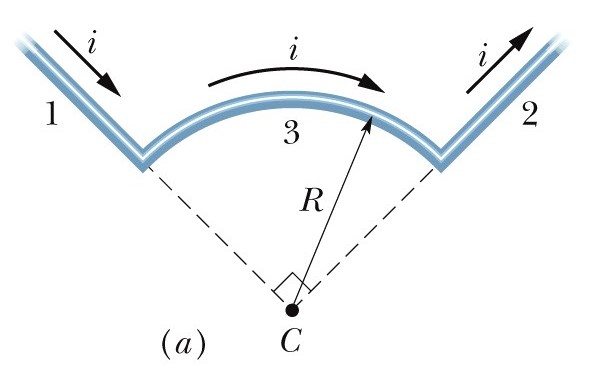
\includegraphics[width=0.5\textwidth]{halliday_10e_fig_29_08.jpg} % here is where you include the filename and how wide you want the image to be. The file name is case sensitive and the extension matters. The width is set as a fraction of the width of the text on the page. I have set the default to be 50% of the text width but you can change it to whatever suits your purpose.
        \caption{You may insert an optional caption here}
        \label{fig:example}
    \end{center}
\end{figure}

\end{document}
